\documentclass{article}
\usepackage[utf8]{inputenc}
\usepackage{geometry}
\usepackage{graphicx}
\usepackage{pgfplots}
\usepackage{amsmath}
\usepackage{amssymb}
\usepackage{amsfonts}
\usepackage{mdframed}
\usepackage{amsthm}
\usepackage{tikz}
\usepackage{multicol}

\geometry{a4paper, left=2cm, right=2cm, top=1cm, bottom=2cm}

\pgfplotsset{compat=1.18}
\begin{document}

\begin{minipage}{0.7\textwidth}
    \small \textbf{LABORATORIO DE MECÁNICA VECTORIAL}  \\
    \small {Facultad de Ciencias, Universidad Nacional Autónoma de México} \\
    \small {Profesor: Radamés Ricardo Reynoso Manríquez} \\
    \small {Ayudante: Ana Laura Córdova Lara}\\
    \small {Fecha de entrega: 13 de Febrero de 2024} \\
    \small {Nombre completo: Andrés López González} \\
    \small {Tarea número I}
\end{minipage}
\hfill
\begin{minipage}{0.12\textwidth}
    
\includegraphics[width=\linewidth]{logo_universidad}
\end{minipage}

\section*{Cuestionario I}

PREGUNTA 1. Defina exactitud de medición.\\\\
\textit{La exactitud de la medición se refiere a la cercanía entre el valor medido y el valor verdadero o aceptado de una magnitud física. Es decir, se trata de cuán cerca está el resultado de una medición del valor real o verdadero de la cantidad que se está midiendo. La exactitud se evalúa mediante la comparación del resultado de la medición con un valor de referencia conocido o aceptado (normalmente verificable teóricamente dependiendo la complejidad del caso).}\\\\

\textit{De manera aplicada... si estamos midiendo la longitud de un objeto con una regla calibrada, y el valor verdadero de la longitud del objeto es 10 centímetros, la exactitud de nuestra medición dependerá de qué tan cerca esté nuestra lectura de la regla del valor verdadero de 10 centímetros. Si nuestra medición es de 9.8 centímetros, podemos considerarla como bastante precisa (en un momento veremos qué es esto) y con alta exactitud. Sin embargo, si la medición es de 11 centímetros, la exactitud de la medición sería baja, ya que la medida está bastante alejada del valor verdadero (incerditumbre de un centímetro). Es importante que además de la dispersión (que veremos adelante en la precisión) también haya exactitud, pues nos da un mejor acercamiento al valor real de la medida.}\\\\


PREGUNTA 2. Defina precisión en la medida. \\\\
\textit{La precisión de la medida se refiere a la capacidad de un instrumento de medición para proporcionar resultados consistentes y repetibles cuando se mide una misma cantidad en condiciones similares. En otras palabras, la precisión se relaciona con la dispersión de los resultados obtenidos al realizar múltiples mediciones del mismo objeto bajo las mismas condiciones.} \\\\

\textit{Un instrumento de medición se considera más preciso cuando las mediciones repetidas producen resultados cercanos entre sí. La precisión no está necesariamente relacionada con la exactitud, ya que un instrumento puede ser preciso pero no necesariamente proporcionar resultados cercanos al valor verdadero o aceptado de la magnitud medida.}\\\\

\textit{Ejemplo de ello es si utilizamos una balanza para medir la masa de un objeto varias veces y obtenemos resultados consistentes y cercanos entre sí, podemos decir que la balanza es precisa. Sin embargo, si esos resultados no coinciden con el valor verdadero de la masa del objeto, entonces la balanza no es exacta, pero sigue siendo precisa en términos de repetibilidad de las mediciones. Un ejemplo más complejo es con un espectrofotómetro, dependiendo de la calidad de este y los "multiplicadores" de las ondas electromagnéticas emitidas por el objeto de estudios obtendremos señales eléctricas muy (o poco) fidedignas del compuesto.}\\\\

PREGUNTA 3. Para saber el tamaño al que crecen naturalmente las hojas de un
árbol se hicieron mediciones que arrojaron una longitud promedio de L = 8.32 cm,
con desviación típica de 0.53 cm. ¿Cuál es el intervalo de confianza en el cual se
encuentran el 68\% de las medidas?\\
\textit{Estamos buscando el intervalo de confianza que cubre  hacia ambos lados de la media 68\%, esto quiere decir que respecto a la recta simétrica de nuestra distribución normal habrá un 34\% de confianza hacia cada lateral. Esto por definición siempre es un sigma, o lo que quiere decir de forma menos ambigua es que al desplazarnos hacia la izquierda o derecha para obtener el primer 34\% de confianza (teniendo nuestro origen en la mitad de la gráfica), este primer 34\% es lo referente a un sigma, como si reglaramos el plano en términos de \sigma en lugar de unidades.}
\newpage

\textit{Dado que la desviación estándar es de 0.53 cm, podemos calcular el intervalo de confianza sumando y restando esta desviación estándar a la media. Lo definimos de la forma siguiente tal que x = longitud esperada de la hoja dentro del intervalo de confianza:}
\begin{align*}
    B_L(x,\sigma) &= x \in [L-\sigma,L+\sigma]\\
    &= x \in [8.32cm - 0.53cm , 8.32 cm + 0.53 cm]\\
    &= x \in [7.79 cm, 8.85 cm]
\end{align*}

PREGUNTA 4. Para determinar el volumen de un cilindro ($V = \pi r^2h$), se midió el
radio de la base y se obtuvo r = (1.83 + 0.05) cm, y para la altura h = (5.60 + 0.05)
cm.\\
a) ¿Cuál es la incertidumbre combinada correspondiente al volumen? $\Delta V \approx 3.7455481cm^3 \cong 3.74 cm$\\
b) ¿Cuál es la incertidumbre relativa porcentual asociada al volumen del cilindro? 6\%\\
\begin{figure}[h]
    \centering
    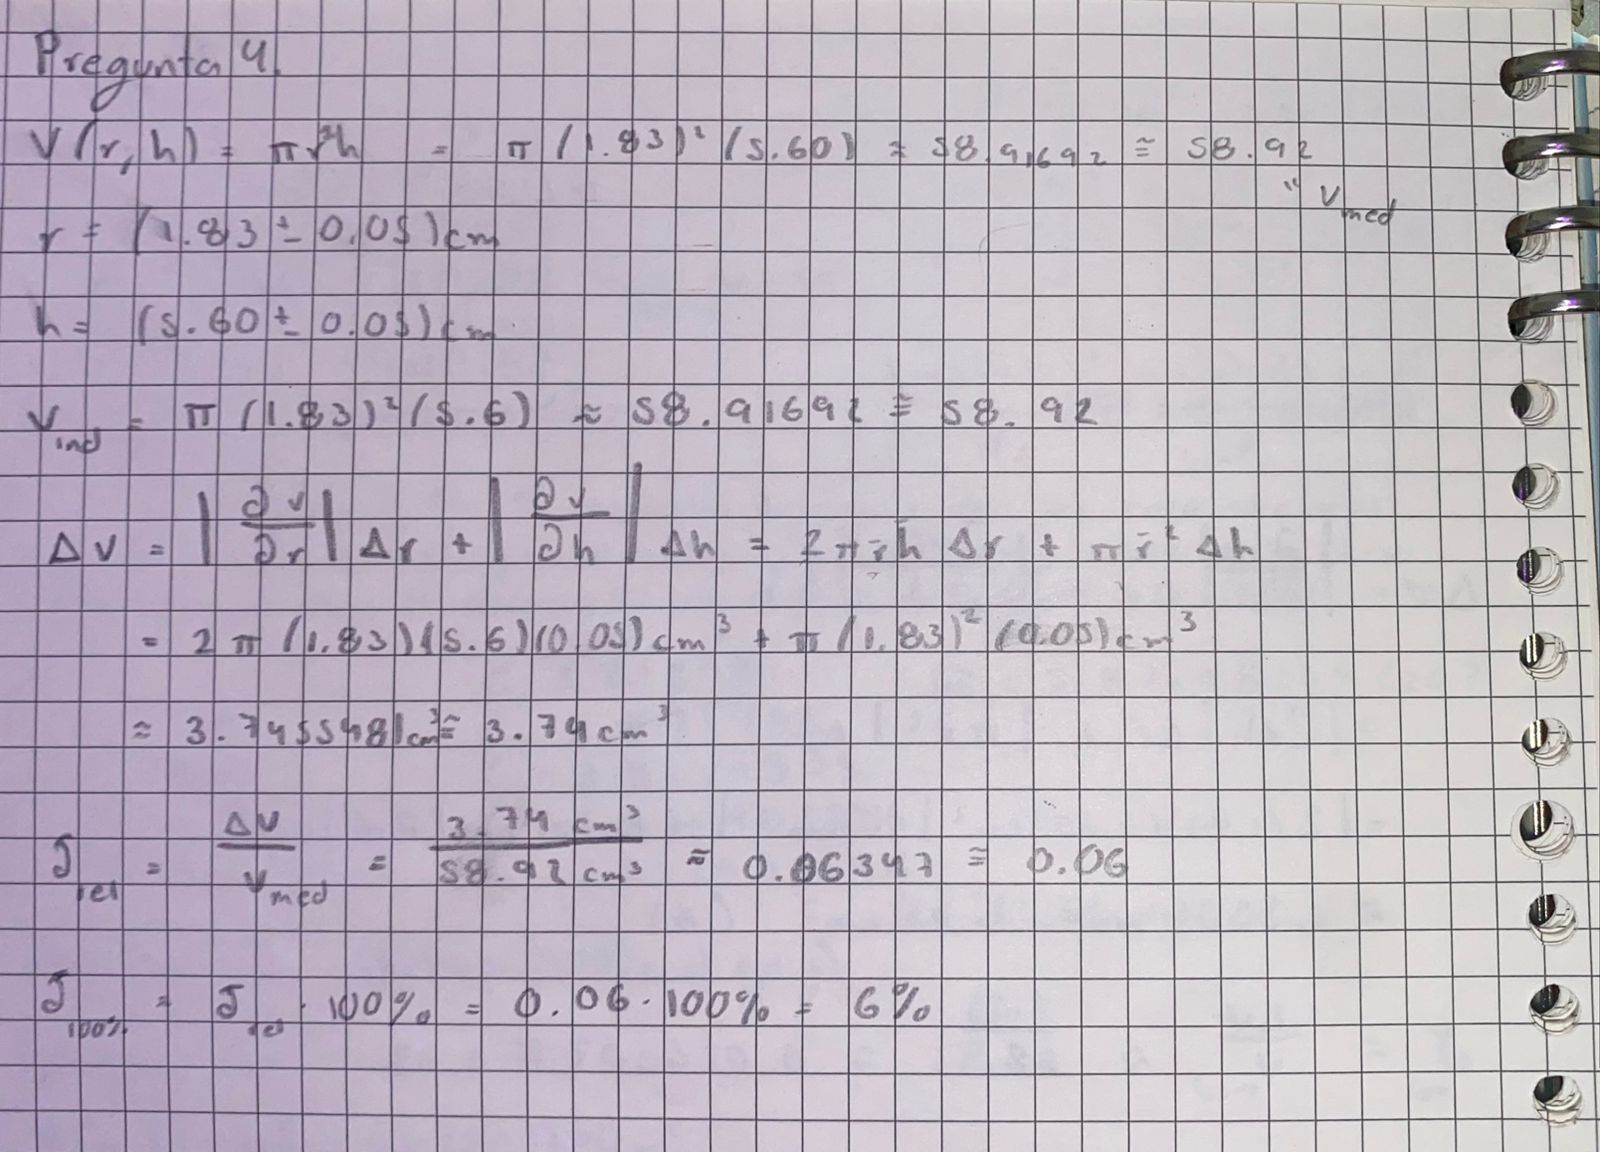
\includegraphics[height=10cm]{cuatroej.jpeg}
    \caption{Procedures (Ej. IV).}
    \label{fig:cuatroej}
\end{figure}
\\\\
PREGUNTA 5. ¿Cuáles son los parámetros estadísticos que nos proporcionan
información sobre la tendencia central de un conjunto de datos? Define cada uno de
ellos.\\\\
\textit{El promedio siendo este el más conocido, también nombrado como media, representa el valor típico o central de un conjunto de datos y se calcula como la suma de todos los valores dividida por el número total de valores [$n^{-1} \cdot \sum_{i=1}^n x_i$]. La mediana (que aunque no se haya abordado) es el valor que ocupa la posición central en un conjunto de datos ordenados de menor a mayor, dividiendo el conjunto en dos partes iguales, esta es extremadamente imprecisa porque no distingue en absoluto la dispersión de los datos. La moda (tampoco vista pero de las 3 parámetros más reconocidos de tendencia estadística) es el valor que aparece con mayor frecuencia en un conjunto de datos, aunque no todos los conjuntos la tienen y algunos pueden tener más de una moda. La desviación estándar o típica indica cuánto se alejan los valores individuales de la media, se calcula como la raíz cuadrada de la varianza, mientras que el promedio se aplica al ser hasta 10 datos con los que trabajamos, la desviación estándar se aplica al ser mayor o igual a 10 cantidades pues nos proporciona una mucho mejor noción de lo que es la dispersión de datos respecto a una recta hipotética que generan estos mismos datos. Otros datos relevantes en estos parámetros son las incertidumbres ya que nos aproximan cuánta es la varianza de un dato, la incertidumbre absoluta es la diferencia entre el valor medido y el valor verdadero de una magnitud, mientras que la incertidumbre relativa es la incertidumbre absoluta dividida por el valor verdadero de la magnitud, expresada como un porcentaje. La incertidumbre asociada se estima a partir de la experiencia y el conocimiento del proceso de medición, y se utiliza para expresar la confianza en el valor medido. Por último, la incertidumbre indirecta se calcula a partir de las incertidumbres de otras magnitudes medidas que están involucradas en su determinación, involucra una función multivariable y derivadas parciales para su deducción.}
\end{document}
